\section{Data generation}\label{sec:data_gen}
As we could not find a dataset that matches our requirements, we generate a new dataset using competition result published by the DSV (Deutscher Schwimm-Verband e.V.). All swimmers that are eight years or older and take part in competitions in Germany must register at the DSV. The DSV publishes all official competition results as well as information about registered swimmers online \footnote{\url{http://www.dsv.de/schwimmen/wettkampf-national/schwimmerabfrage/}, accessed 02.01.2020}; thus, we can access a considerable amount of data for our dataset.\\
Similar to the records in \textit{Prediction on Performance of Age Group Swimming Using Machine Learning} by \citet{Xie.2015} our dataset contains records that look like this: \texttt{(gender, age, training age, 50m time, 100m time, 200m time)}. To get a continuous representation of our data, we express all times in seconds with two decimal places.\\
We include the gender and the age of the swimmer as boys and girls develop differently at different ages. \citet{Golle.2015} showed in their study that the fitness performance improves when children get older. While boys outperformed girls of the same age-group in upper-extremity muscular power and endurance, girls performed better in flexibility test. All of the three aforementioned physical aspects are important for swimmers; thus, we expect different performances by swimmers of different age groups and gender. We use the swimmer's age group to determine his age instead of his actual age at the respective competition. Our dataset covers ages from nine to 14 years\\
The training age describes how long the swimmer has been training competitive swimming. The longer the swimmer has been training, the better is the swimmer's endurance and his technique as explained in section \ref{sec:sport_theory}. On top of that, he gained experience in competitions; thus, he may be less nervous during competition. In our dataset, we consider training ages ranging from one to seven years.\\
\citet{Wakayoshi.1992} have shown that for college swimmers, the distance and the corresponding time have a linear connection thus we can calculate the longer distance time based on any shorter distance. However, \citet{Golle.2015} observed a curvilinear improvement in upper-body strength and endurance for older junior swimmers. Putting this together, we expect the correlation between 50m, 100m, and 200m time to be non-linear, dependent on the age, training age and gender of the swimmer.\\
Using the aforementioned considerations, we generate two different datasets, a training and a test dataset. The training dataset consists of 116 samples with 49 female and 67 male swimmers. The test dataset contains 19 samples, ten of which are female. The swimming times in the dataset were achieved at the same competition on the same weekend in a 25m pool.
\begin{figure}[ht]
    \centering
    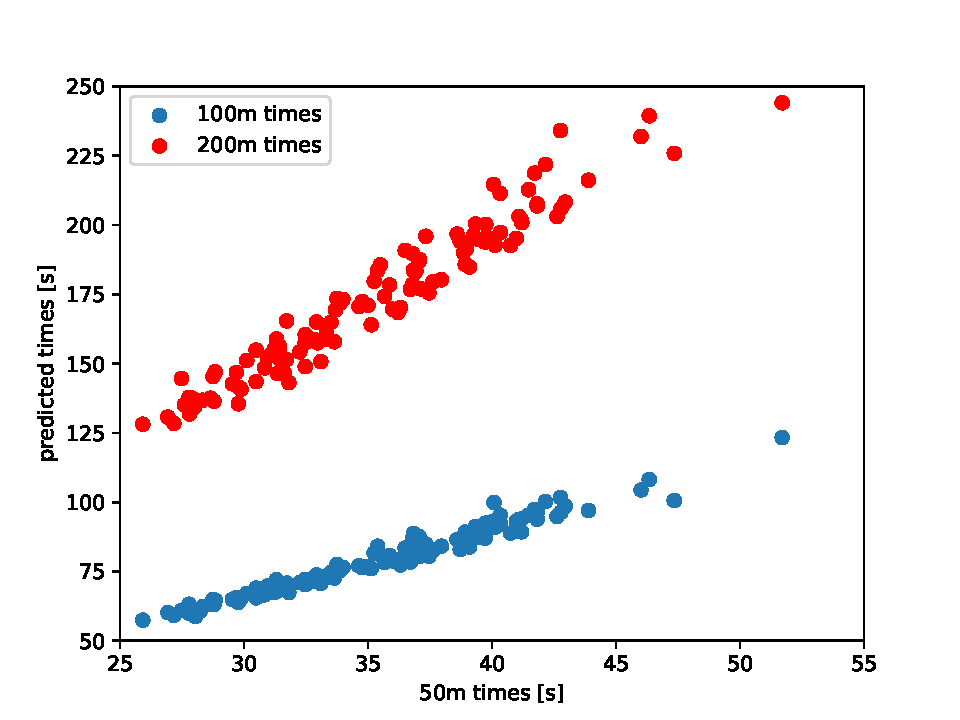
\includegraphics[scale=0.5]{visualisation/training_data.pdf}
    \caption{Training data: correlation of 50m and longer distance times}
    \label{fig:training_data}
\end{figure}
Figures \ref{fig:training_data} and \ref{fig:test_data} show the correlation of 50m and the longer distance times. In order to plot the samples in 2D, we omit the information about the swimmer. We can see that the times have a strong linear correlation with a Pearson correlation coefficient of $0.983$ for the 100m training data and $0.972$ for the 200m training data. Therefore, our initial assumption that age is essential for the prediction was wrong. Even for junior swimmers, the times follow a linear correlation as introduced by the critical power concept in section \ref{critical_power}, independent of the age, the training age or the gender.\\
\begin{figure}[ht]
    \centering
    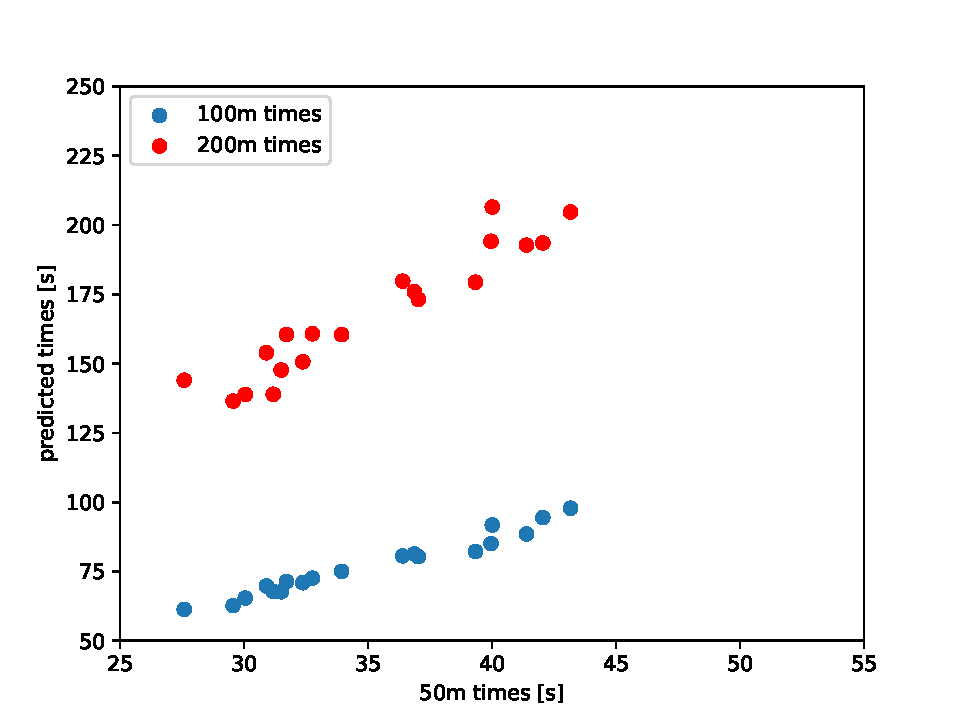
\includegraphics[scale=0.5]{visualisation/test_data.pdf}
    \caption{Test data: correlation of 50m and longer distance times}
    \label{fig:test_data}
\end{figure}
Also, we observe a higher variance in the long-distance times for higher 50m times. As we can see in Figure \ref{fig:training_age}, these higher 50m times are mostly from swimmers that are in their first or second training year. These swimmers have less competition experience or a rather bad technique. Moreover, young swimmers are often very nervous at competitions; thus, they make mistakes more likely. This makes it harder to predict their performance. The better a swimmer is, i.e. the longer he trains and the better his technique is, the more reliable his performance will be.
\begin{figure}[ht]
    \centering
    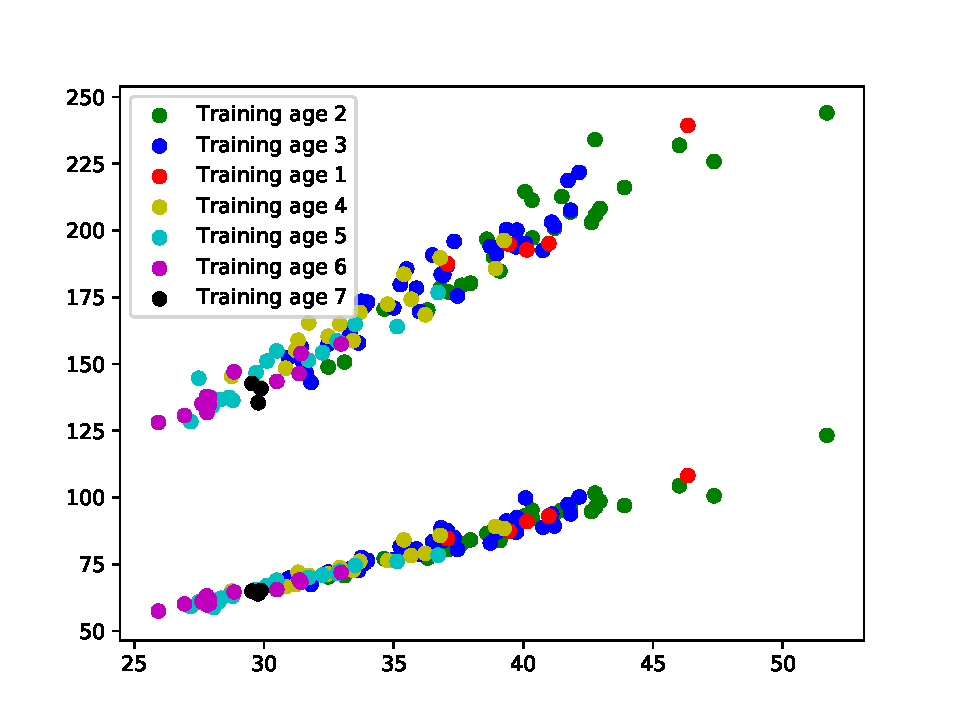
\includegraphics[scale=0.5]{visualisation/training_data_train_ages.pdf}
    \caption{Training data: influence of training age}
    \label{fig:training_age}
\end{figure}